\section{Installation av Gloria}
På Gloria så finns det en huvudenhet, en \textbf{beagleboard} (markerat 1 i figur 1), som innehåller all styrlogik som låter användaren hantera roboten. Beagleboardet har ett antal USB-portar, varav en är ansluten till en blåtandsdongel (markerat 2 i figur 1) som låter användaren ansluta direkt till beagleboardet från godtycklig pc.

\begin{figure}[h!]
	\center
	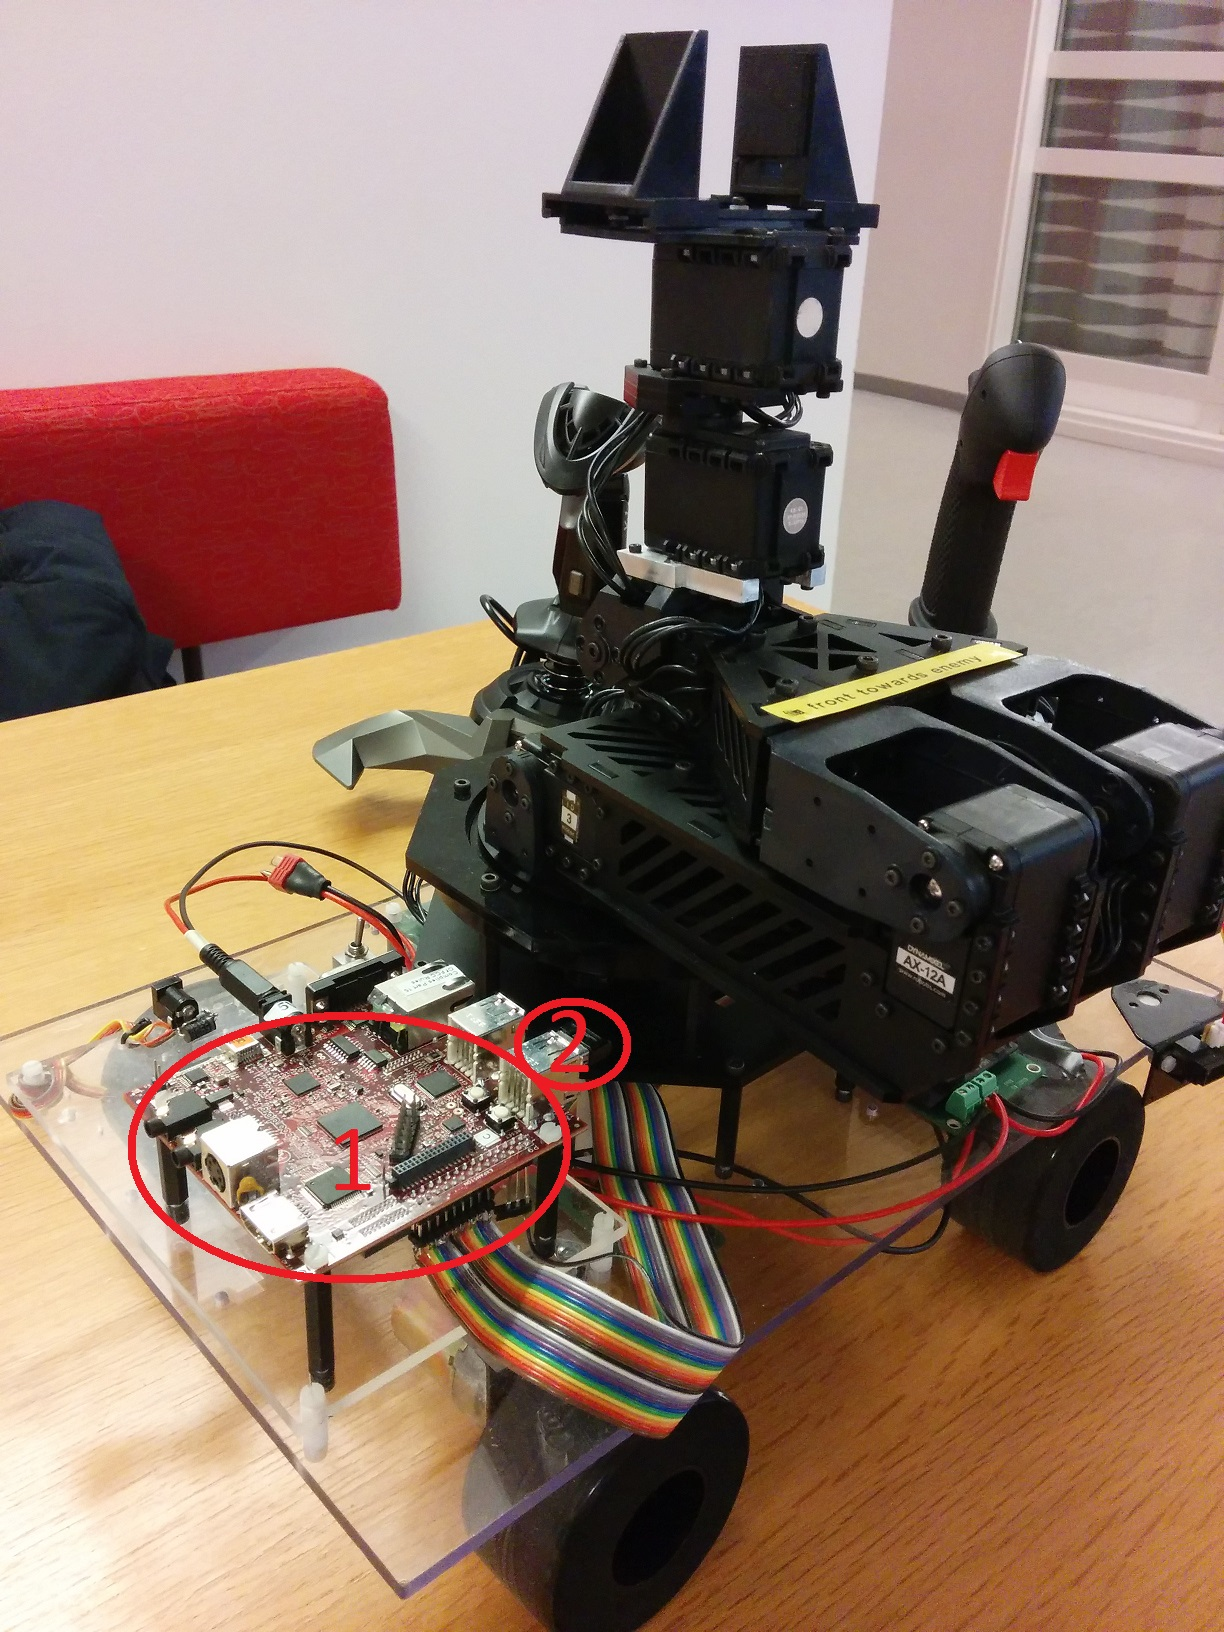
\includegraphics[scale=0.2]{GloriaAnvh.jpg}
	\endcenter
	\caption{Figur 1. Gloria snett bakifrån.}
\end{figure}
\newpage
\subsection{Ansluta till Gloria}
För att kunna ansluta till huvudenheten behöver följande göras (antag att man sitter på en linuxmaskin):
\begin{enumerate}
	\item Ha tillgång till en terminal på huvudenheten, det enklaste är att ansluta en skärm och tangentbord till den.\newline Lösenordet är \textbf{temppwd}
	\item Kör \textbf{sudo bluez-simple-agent hci0 xx:xx:xx:xx:xx:xx} där man byter ut kryssen mot den anslutande blåtandenhetens mac-adress.
	\item Upprätta en förbindelse från den anslutande PCn till huvudenheten. Huvudenheten är listad som arm-0 via blåtand.
	\item Kör \textbf{sudo bluez-test-device trusted xx:xx:xx:xx:xx:xx yes} på huvudenheten där man återigen byter ut kryssen mot blåtandenhetens mac-adress.
	\item Man kan nu ta bort förbindelsen (men låt blåtand fortsatt vara påslaget) från den anslutande PCn.
	\item Kör \textbf{sudo pand -n -c 00:19:0E:0F:F0:6F	} på den anslutande PCn.
	\item Kör \textbf{sudo ifconfig bnep0 192.168.99.2 up } på den anslutande PCn.
\end{enumerate}
Nu borde man kunna pinga och ssha in på ubuntu@192.168.99.1 vilket är huvudenhetens statiska ip-adress. I framtiden behövs bara de två sista stegen genmföras.
\subsection{Starta Gloria}
\begin{enumerate}
	\item Om anslutning har etablerats till roboten så behöver man hitta filen mainThread.py som ligger i usr/bin/home/main.
	\item Kommandot för att starta systemet är \textbf{python mainThread.py}
	När detta kommandot körs så sätter systemet igång och roboten lägger sig i vänteläge.
	\item Efter att mainThread.py har startats på roboten så startar man upp en ny terminal lokalt på datorn som roboten ska styras ifrån och hittar Gui.py. Sedan kör man kommandot: \textbf{python Gui.py}
	\item Anslut två joysticks via USB (till PC). För att styra motorn behöver du en mad catz och för armen du en Saitek.
\end{enumerate}
\subsection{Kort om AVR}
Eventuell mjukvaruuppdatering kan installeras via JTAG-porten.
\newline
För att starta om AVR så finns det en blå knapp tillgänglig bredvid processorn på virkortet. PCB kan på samma sätt startas om med en grå knapp.
\newpage
